\section{Decay Spectrometer}
\label{DecaySpectrometer}
\subsection{Overview of re-optimized Decay Spectrometer}

The SHiP Decay Spectrometer (DS) consists of large vacuum vessel, Surround Background Tagger (SBT), Main Spectrometer Tracker (ST), including a large spectrometer magnet with a total field integral of XX Tm, Timing Detector (TD), Calorimeter and downstream Muon systems.

DS has to perform precise measurements of tracks and photons originated from decay vertices of hidden particles in the decay volume, measure their momenta, and provide PID information. Moreover DS has to ensure a redundant background suppression using timing and tracking information from TD and SST, vetoing criteria from SBT, and PID by the calorimeter system and muon detector. 

This section describes the principal features and main parameters of the DS sub-detectors as implemented in the FairSHiP. The parameters have used in the simulation studies of the DS performance reported in section \ref{DSperformance}. Specific proof-of-principle tests of prototypes have been undertaken which demonstrate that the parameters listed can be achieved.

\noindent {\bf SBT}\\
\noindent
SBT detects charged particles either entering the vacuum vessel from outside, or produced in the inelastic interactions of muons and neutrinos inside the vacuum vessel walls. Compared to the TP there are currently two options of the SBT under consideration: a new plastic scintillator (PS-SBT) option, and the liquid scintillator (LS) detector (LS-SBT) which remains the baseline with the LS of linear alkybenzene (LAB) and 2.0 g/l diphenyl-oxazole (PPO) as the fluorescent.

The LS-SBT is sub-divided in individual cells integrated to the support structure of the vacuum vessel. Accordingly, the cell size is 80 cm in the longitudinal direction and typically O(120 cm) in the transverse direction, depending also on its z-position. The thickness of the LS layer, surrounding the side walls of the complete decay vessel up to XX cm and enclosed by a YY cm thick outer steel wall, is 30 cm. Due to the conical shape of the decay vessel the LS volume of O(243 m$^3$) is significantly reduced compared to the TP.  This allowed to increase the PPO concentration from 1.5 g/l quoted in the TP without any increase in price for the LS.
%
\begin{figure}[h]
\centering
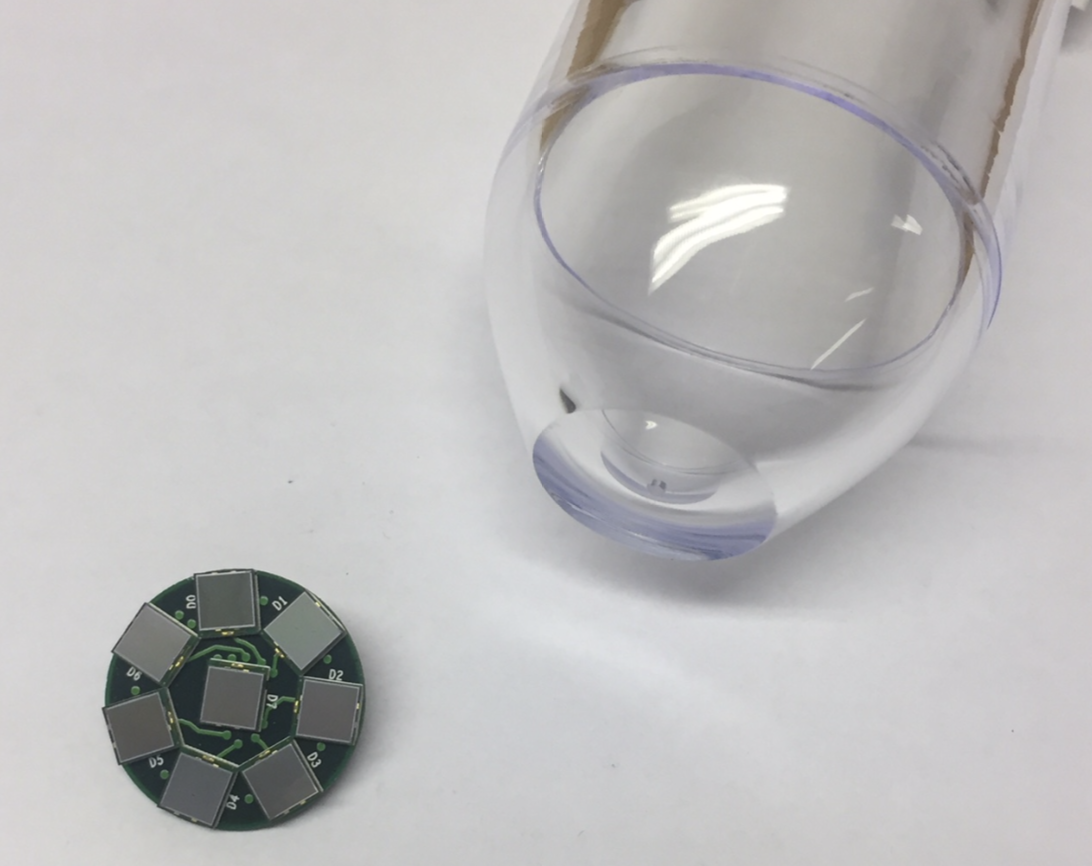
\includegraphics[width=0.35\columnwidth]{figs/DecaySpectrometer/WOM.png}
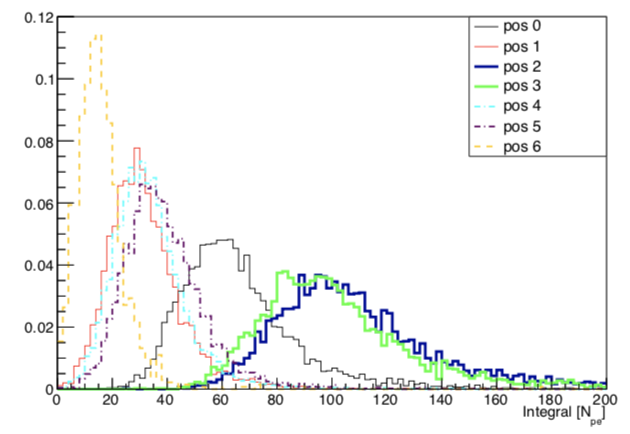
\includegraphics[width=0.45\columnwidth]{figs/DecaySpectrometer/SBT.png}
\caption{Left: prototype of a WOM MODULE, tested at the T2 H2 CERN-SPS area.
  Right: Number of photoelectrons detected by the WOM module for muons at different beam positions.}
\label{fig:SBT}
\end{figure}
%
Each cell of the LS-SBT is readout by two wavelength-shifting optical modules (WOM) detecting the scintillation light emitted in the range between 340 nm and 400 nm and transporting the light to a ring of 24 SiPMs of 3 x 3 mm$^2$ area directly coupled to the WOM tube. There are O(2000) WOMs for the whole LS-SBT. Test beam measurements in 2017 using a cell with a volume of 50 x 50 x 30 cm$^2$ (and 1.5 g/l PPO) show that a detection efficiency for muons of at least 99.6\% is achieved, if one WOM (equipped with a lightguide and viewed by an array of eight 6 x 6 mm$^2$ SiPMs, as shown in Figure\ref{fig:SBT}, left) is required to detect at least five photoelectrons. The average number of photoelectrons detected by this WOM depends on the position of the particle traversing the LS cell and was measured to be at least 30 (see Figure\ref{fig:SBT}, right). The measurements also demonstrate that a time resolution of 1 ns is achieved when two WOMs with a threshold of two photoelectrons are required.
Since the WOM-based LS-SBT principle has been demonstrated to work with good performance, the option with large-area PMTs is currently not further pursued. 

Several improvements (like increasing the PPO concentration and the direct coupling of the SiPMs to the WOM tube without using a lightguide) to increase the detected light yield and hence the efficiency have been identified, which can also improve the time resolution due to the higher photoelectron statistics. The new design will be tested in a testbeam measurement in October 2018 using a larger cell size of 120 x 80 x 30 cm$^3$. These testbeam measurements will also test a small-scale version of the LS filling system and first versions of the two readout-electronics options. Moreover, first studies will be performed whether individual SiPM readout provides any information on the original direction of the primary scintillation photon hitting the WOM tube.

While the basic components of the LS mixture have been identified (solvent LAB, fluor PPO), the exact composition still has to be optimized to the dimensions of the SBT cells. This concerns the concentration of PPO and a possible addition of paraffin oil to increase transparency vs. scintillation light yield. Reflective coating covering the inner walls of the cells have to be selected based on material compatibility and spectral reflectivity. Moreover, we will test vitamin C as an additive to improve the chemical durability of the LS towards accidental exposure to atmospheric oxygen. Finally, the use of green-sensitive SiPMs would allow to use a green dye in the WOM coatings and in turn to add a further wavelength shifter (bisMSB) to the scintillator, improving transparency and thus light response homogeneity. 

In FairSHiP, the cell geometry is implemented and the LS-SBT detector response provides the energy deposit from charged particles inside each individual cell. In the data analysis, a minimum amount of energy deposition (typically 45 MeV, which is slightly below the energy deposition of a MIP traversing a LS cell perpendicular to the vacuum vessel wall) is required to consider a LS cell as fired. Timing information taking into account testbeam results have not been yet implemented in the LS-SBT response.

The information of the LS-SBT has been used in background suppression studies of DIS events in the decay-vessel walls induced by either neutrinos or muons, assuming that the detection probability inside a LS cell of charged particles depositing at least 45 MeV is 99.9\%. The testbeam measurement results are already very close to this value. (In future studies, the energy threshold in the individual cells will be lowered, e.g. to 10 MeV, and instead it will be required that the sum of energy depositions in adjacent LS cells is above a certain threshold of O(45 MeV), since the energy deposition of one particle in the SBT is not necessarily contained in one SBT cell.)

\noindent {\bf ST}\\
\noindent
The purpose of the SHiP Spectrometer Tracker\footnote{%
   The SST was called Hidden Sector spectrometer in the Tecnhical Proposal.
   }
(SST) 
is to reconstruct with high efficiency the tracks
of charged particles from the decay of hidden particles, while rejecting background events.
Additionally, the SST must provide an accurate determination of the track
momentum and of the flight direction within the fiducial decay volume.
The precision of the extrapolated position of the tracks must be well matched with the
segmentation of the timing detectors (see section~\ref{sec:timing_detectors}) such that
the high accuracy of the associated track time can be used to remove combinatorial background.
The invariant mass, the vertex quality, the timing, the matching to background taggers
and the pointing to the production target are crucial tools for rejecting background. 
% from spurious $V^0$ meson decays, neutrino interactions or from random combinations.

The spectrometer consists of a large aperture dipole magnet  
%(discussed in Section~\ref{sec:spectrometermagnet})
and two tracking telescopes on each side of the magnet, 
%A layout with four tracking stations symmetrically arranged around the dipole magnet,
%as depicted in Figure~\ref{fig:spectrometer-layout},  is taken as a baseline.
%The size and layout of the tracker stations is connected to the size of the magnet.
%A dipole spectrometer magnet with a horizontal gap of 5~m, a height of 10~m
%and a length of 5~m provides good acceptance coverage and is considered
%feasible at a reasonable cost. % (see section \ref{sec:spectrometermagnet}).
%The $B$ field is about 0.14~T at its maximum and about 0.08~T at the location of the
%closest tracker stations, just outside the magnet.
%On the longitudinal axis the field integral between the second and third station
%is approximately 0.65~Tm.
each composed of two tracking stations. 
The four stations are identical with a nominal acceptance of 5~m in X and 10~m in Y
and based on ultra-thin straw drift tubes oriented horizontally.
Each station contains four views, in a Y-U-V-Y arrangement, where U and V are stereo views
with straws rotated by a small angle $\pm\theta_{\rm stereo}$ around the Z axis with respect to
the Y-measuring straws.
The straw veto station at the beginning of the hidden sector decay volume was removed
after demonstrating that no loss in performance of background rejection could be obtained by using 
other detector information, see section~\ref{sec:background_studies}.

The main change since the TP is the increase of the straw diameter $D$ from 10~mm to 20~mm.
This change is motivated by the refined background rate simulations (see section \ref{sec:background_rates}) 
which confirm that for $D=20~$mm the rate per straw remains modest ({\color{red}XXX~kHz TO BE CHECKED} 
in the hottest straw).
Tools for producing 20~mm straws were developed and several prototype straws,
using as before a $36~\mu$m thick PET film coated with 50~nm Cu and 20~nm Au,
were produced with no new difficulty encountered compared to fabrication of 
the original 10~mm straws. 
Several straws of 20~mm diameter and 5~m length were fabricated.
The rupture overpressure was measured on ten samples of 50~cm length and,
as shown in Fig.~\ref{fig:rupture_pressure_straws_D20mm}, was found to be around 4.4~bar, 
as expected.
% TEMUR: confirm overpressure! 
This is considered a sufficient margin for operating the straws at a pressure of about 1~bar in vacuum.
The torsion of 5~m long straws, cemented on one side and pressurized to 1~bar overpressure,
was measured and a rotation of 38 degrees was found at the free end.
A torque of about $0.076~{\rm N\,m}$  was needed to cancel the rotation.
A 2~m long $D=20~$mm straw was fabricated  and its performance as a MIP detector
was characterized in a testbeam run in the SPS north area 
as a function of wire offset at nominal conditions ($\sim 1.05$~bar pressure, 
70\% Ar / 30\% CO$_2$).
First results indicate that a straw hit resolution of $120~\mu$m is achievable with high 
hit efficiency and over most of the straw diameter, independently of the wire offset,
as visible in figure~\ref{Fig:straw_resolution_TB2017}.
The drift time spectra for different wire offsets were analyzed and methods are being investigated
to extract the local wire offset from the distinctive features of the spectra.
Alignment studies for the full detector, using MC simulation, are being started, which should allow
us to define the geometrical constraints for the mechanical engineering design.

\begin{figure}[htb]
\begin{center}
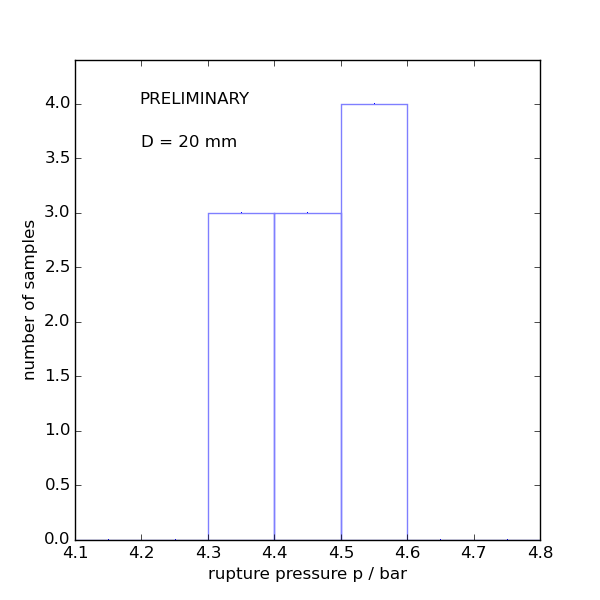
\includegraphics[width=0.5\textwidth]{figs/DecaySpectrometer/rupture_pressure_straws_D20mm.png}
\caption{Rupture overpressure for straw samples with diameter $D=20~$mm.}
\label{fig:rupture_pressure_straws_D20mm}
\end{center}
\end{figure}

\begin{figure}[htb]
\begin{center}
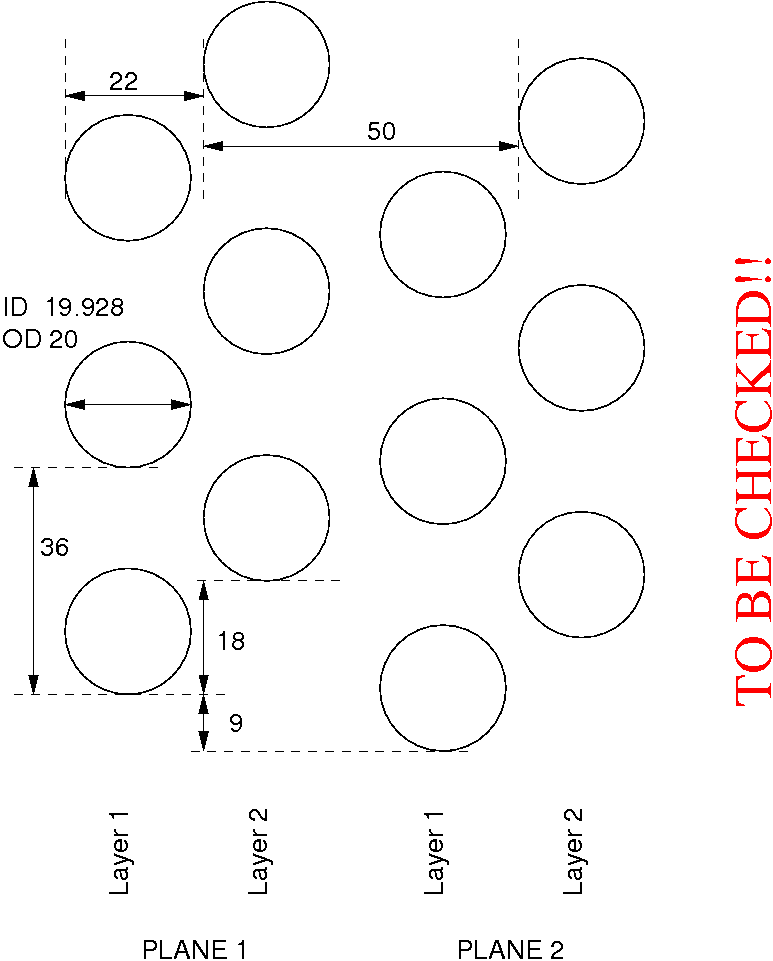
\includegraphics[width=0.5\textwidth]{figs/DecaySpectrometer/straw-layout-SHiP.png}
\caption{New SST straw layout for straw diameter $D=20~$mm as used in FairShip.}
\label{Fig:straw-layout-SHiP}
\end{center}
\end{figure}

\begin{figure}[htb]
\begin{center}
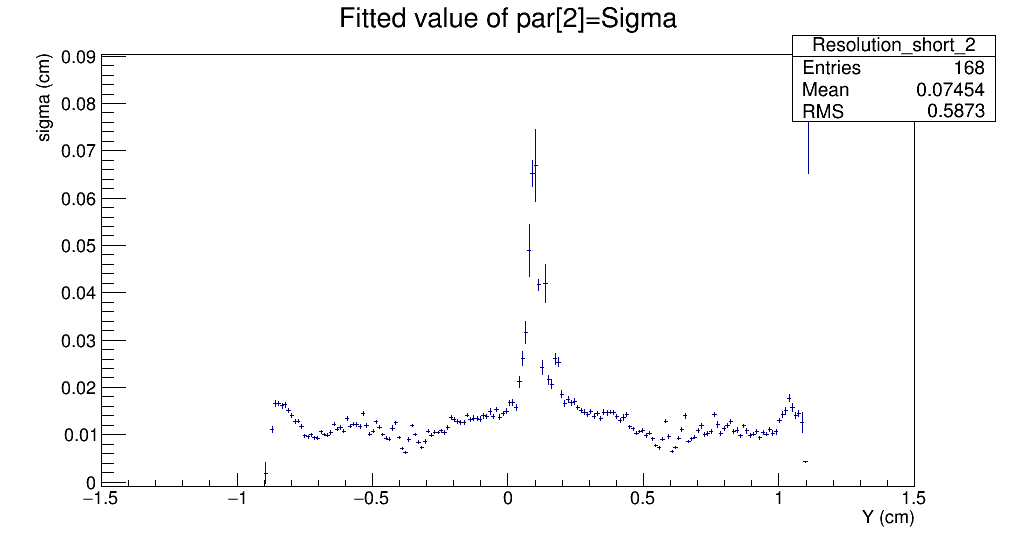
\includegraphics[width=0.45\textwidth]{figs/DecaySpectrometer/sigmaS_328.png} % - the smallest offset 0.02 mm
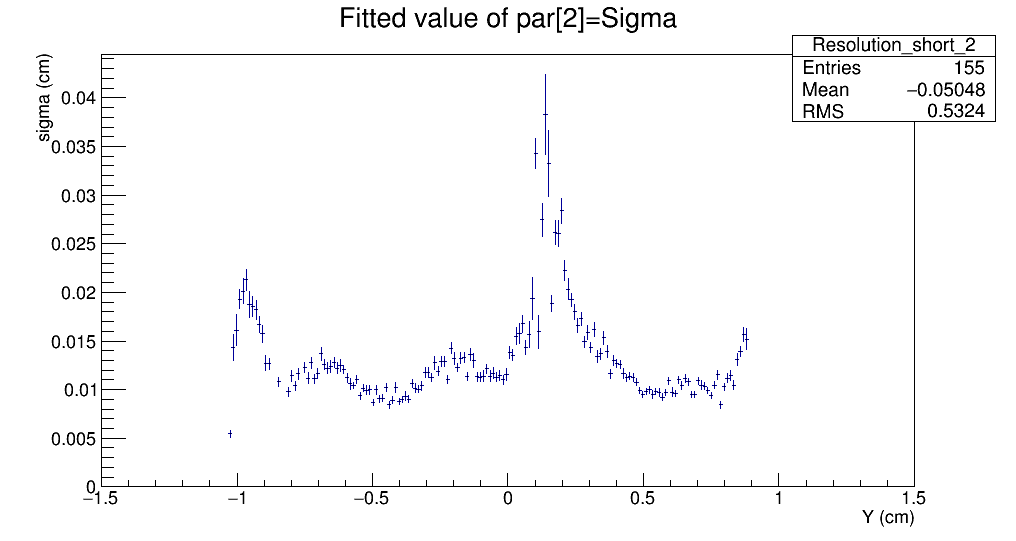
\includegraphics[width=0.45\textwidth]{figs/DecaySpectrometer/sigmaS_163.png} % - the largest offset 1.97 mm
\caption{{\color{red} PRELIMINARY}. Hit resolution across the straw diameter for $D=20$~mm. 
Left: no wire offset. right: wire offset of $\sim 2~$mm.}
\label{Fig:straw_resolution_TB2017}
\end{center}
\end{figure}

Several changes of the SST in FairShip were made and studies are under way.
The straw layout was updated to take into account the larger straw diameter (20~mm), 
see figure~\ref{Fig:straw-layout-SHiP}.
As shown in  section ~\ref{sec:performance}),  the performance of the SST is not degraded 
in comparison to the TP.
Dummy mechanical frames (stainless steel) were added around the straw views, to provide a more realistic
material environment, and it was checked that background rates remain acceptable. 
A new field map, extracted from an FEA calculation, was implemented in the MC simulation, 
including the return field in the yoke. The return field has an effect on the rates
in the last two stations, though these remain acceptable.
An optimization of the station geometry and, in particular, of the stereo angle is ongoing.

The engineering challenges associated with the mechanical properties of strongly tensioned 
long straws and tungsten wires were considered \cite{PietNotes}.
Elongation and relaxation effects, which if neglected would result in excessive
and evolving sagging of the straws, must be taken into account {\sl ab inito} in the design.
Several schemes are being studied, one including a long-stroke constant-force spring,
capable of maintaining the wire under the desired tension while
accomodating a straw elongation of several centimeters, 
and another one utilizing a straw suspension mechanism based on carbon fibres.
A radically different method, developed for the COSY-TOF detector and the PANDA straw  tube 
tracker \cite{PANDA_TDR}, is now also being explored. In this technique, ultrathin straws are held 
together by sparse glue dots in a close-packing configuration and ``inflated'' to 1~bar overpressure.
A self-supporting, rigid an straight straw tube module
can be obtained without externally tensioning the straws and without straw suspension mechanism.

A preliminary conceptual design of the vacuum enclosure is being worked out
which foresees a vacuum chamber with rectangular cross section, longitudinally extending 
over the whole spectrometer length and provided with four rectangular openings on the top side.
These openings are used to lower the tracker station frames, fully equiped, into the vacuum volume.
In this concept, the vacuum enclosure is decoupled from the mechanical structures
for the detector. 
Front-end electronics are located inside the vacuum and require active cooling.

PietNotes:\\
- ``Elastic stability and HEP detectors: a primer'', P. Wertelaers, EP-Tech-Note-2018-005.\\
- ``Anode wire in cylindrical cathode tube : destabilizing electrostatic force'', P. Wertelaers, EP-Tech-Note-2018-003.\\
- ``Pipe regarded as bending beam : destabilizing transverse effect of internal pressure'', P. Wertelaers, EP-Tech-Note-2018-002. 

PANDA:\\
- ``Technical Design Report for the PANDA (AntiProton Annihilations at Darmstadt) Straw Tube Tracker''
   W. Erni et al., Eur. Phys. J. A (2013) 49: 25, DOI 10.1140/epja/i2013-13025-8.\\



Additional pictures:


\begin{figure}[htb]
\begin{center}
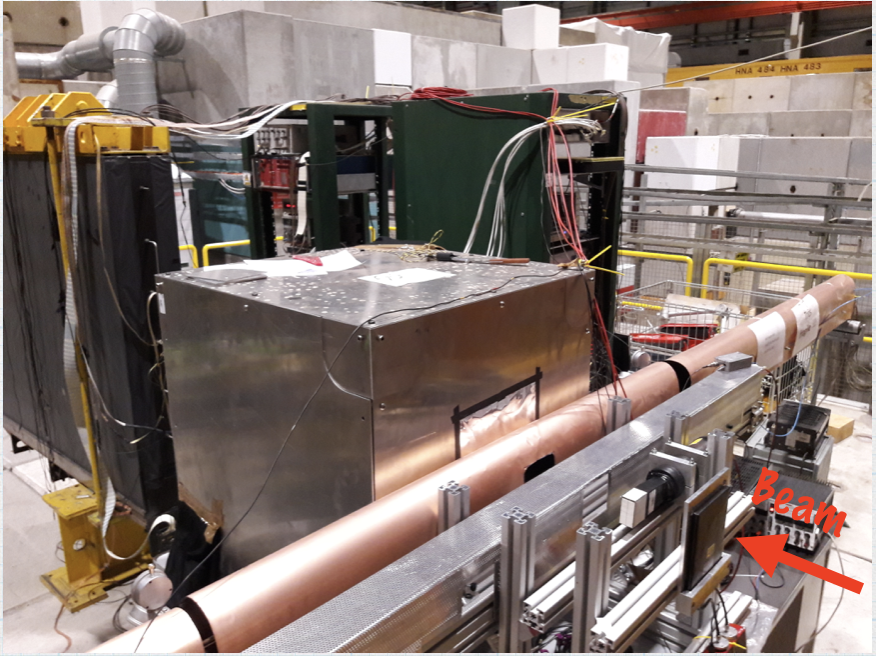
\includegraphics[width=0.45\textwidth]{figs/DecaySpectrometer/SST_TB_setup_2017.png}
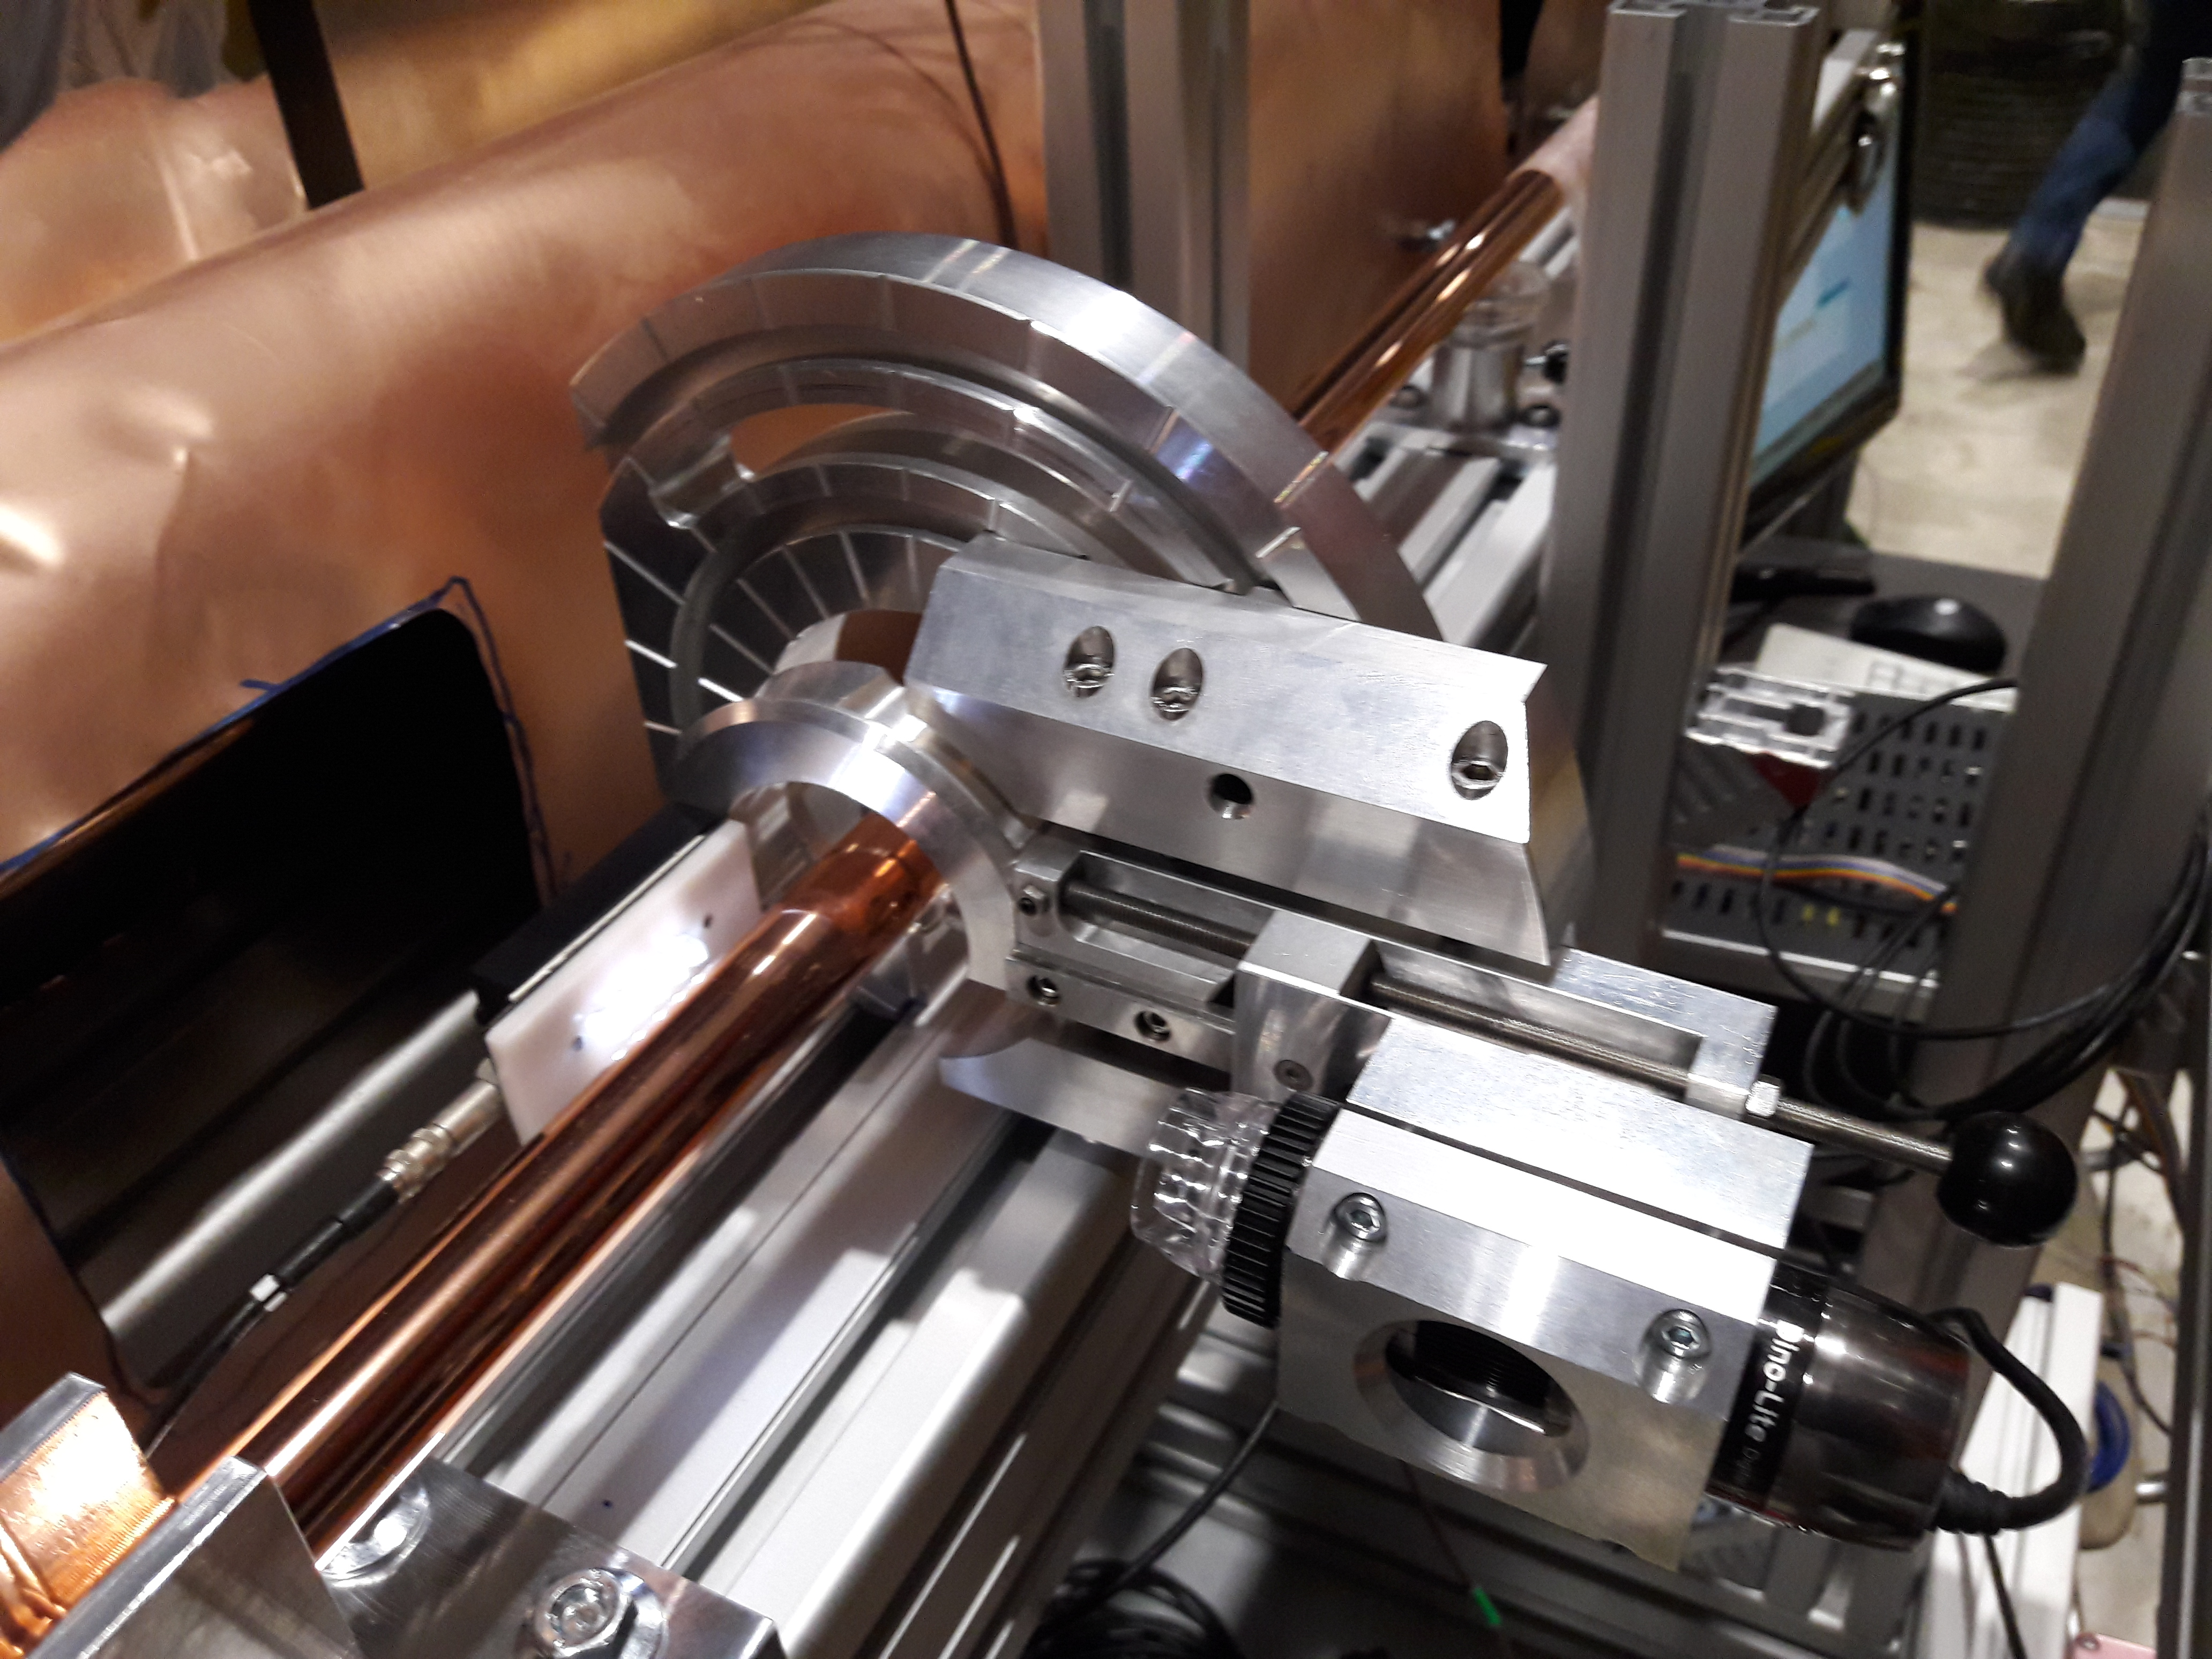
\includegraphics[width=0.45\textwidth]{figs/DecaySpectrometer/20170918_152403.jpg}
\caption{Left: picture of test beam setup. Labels could be added. 
         Right: zoom on straw while wire offset is measured with digital camera.}
\label{Fig:pictures_TB2017}
\end{center}
\end{figure}


\noindent {\bf Timing detector}\\
\noindent
The TP baseline configuration for the plastic scintillator-based option for the SHiP timing detector (TD) consisted of two columns of 305~cm long bars instrumented with PMTs. Although the viability of using large-area SiPMs for the light readout was not known at the time, this scheme was discussed as an attractive one which needed R\&D. It is now demonstrated that the large-area SiPM scheme is not only viable, but actually offers a better performance at a lower cost. A three-column setup of bars read out by arrays of large-area SiPMs is now chosen as the baseline option. 
%
\begin{figure}[h]
\centering
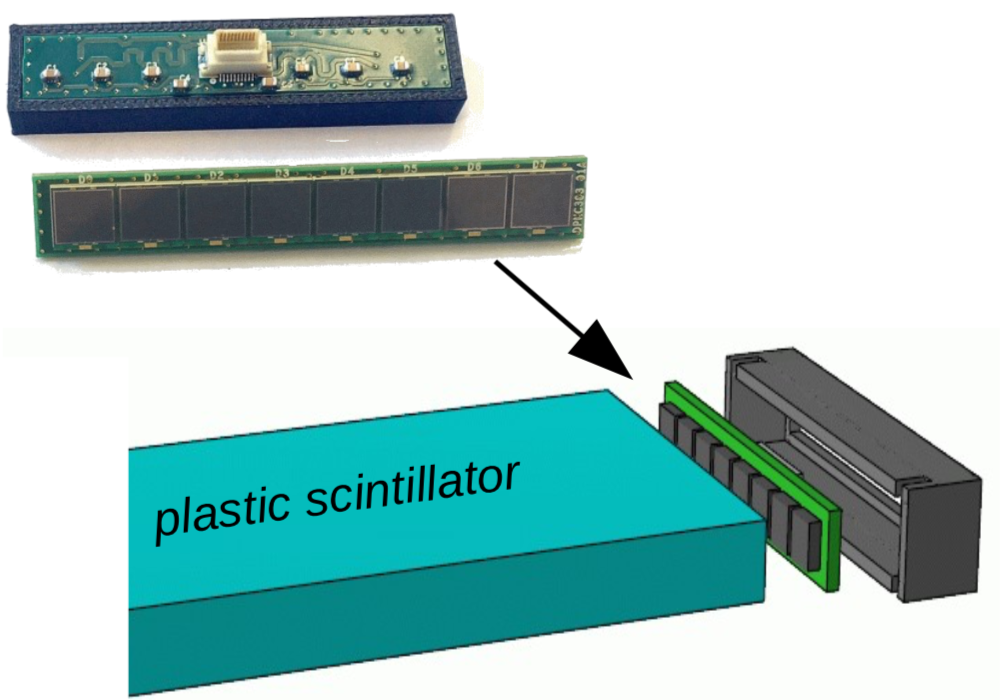
\includegraphics[width=0.35\columnwidth]{figs/DecaySpectrometer/TD_SiPM.png}
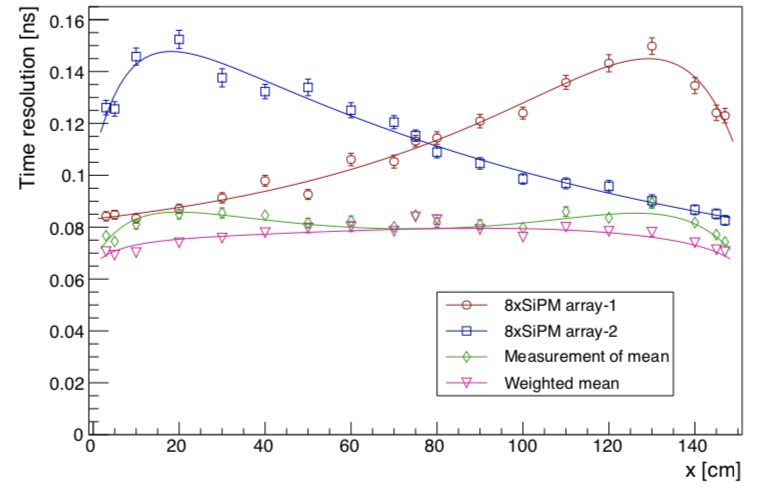
\includegraphics[width=0.55\columnwidth]{figs/DecaySpectrometer/TD_dt.png}
\caption{Left: picture of an array of eight 6~mm$\times$6~mm SiPMs integrated into a PCB with a parallel connection and applied directly to the bar surface. Right: time resolution as measured by the
SiPM arrays at both ends of a 1.5~m bar measured as a function of the beam impact position along the bar~\cite{Betancourt:2017sex}.}
\label{fig:TD}
\end{figure}
%
The current SHiP TD design features bars made of EJ-200 plastic scintillator with dimensions 168~cm$\times$6~cm$\times$1~cm, arranged in three columns and 182 rows with 0.5~cm overlap between bars, for a total area of 5~m$\times$10~m. Each bar is read out on both sides by an array of eight 6~mm$\times$6~mm SiPMs; the signals from the eight SiPMs are summed by an ASIC to form a single channel. Thus there are a total of 564 bars and 1128 channels.  

Figure\ref{fig:TD} presents the results obtained with a 1.5~m long bar read out by two arrays of 8 SiPMs attached to both ends of the bar, as detailed in Ref.~\cite{Betancourt:2017sex}. The resolution of the mean time is demonstrated to be $\sim$80~ps along the whole length of the bar. In Summer 2018, a 22-bar (44 channels) prototype array with 1.68~m long bars (same dimensions as those of the current SHiP TD design) was successfully operated at CERN PS test beams, providing time-of-flight information to a high-pressure TPC prototype. It showed similar timing performance as the single bar over its 2.1~m$ ^2$ active area.

A slightly more modest resolution of $\sim$100 ps has been obtained at the cosmic test of the MRPC prototype representing an alternative option for the TD. 

\noindent {\bf Calorimeter system}\\
\noindent

\noindent {\bf Muon system}\\
\noindent
The muon system has to identify muons with high efficiency ($> 95\%$) and reduce the hadron contamination to less than ${\bf xx} \%$
in a momentum range between $\sim 5-100 $ GeV/c. Moreover it will help the timing detector in rejecting
the combinatorial muon background pairs from the muon halo by requiring a tight ($<$ 1 ns) time coincidence of the two muon tracks:
in fact halo muons are expected to be spread along the whole spill length (1 sec) while muons coming from the same mother particle
are coincident in time.

The muon detector is placed downstream of the calorimeter systems and comprises four stations of active layers
interleaved by three muon filters.
The four stations are 6~m wide, 12~m high  and are placed downstream the calorimeter system.
The amount of material of the calorimeter system corresponds to { 6.7~$\lambda_I$ }. 
The muon filters are iron walls 60~cm thick corresponding to { 3.4~$\lambda_I$ each}.
A muon with normal incidence must have an energy at least of 2.6~GeV/c to reach the first muon station 
and at least 5.3~GeV/c to reach the last muon station.
The multiple scattering of  muons in the material of the calorimeter system and the muon filters drives the 
granularity of the system. Simulation studies show that a readout granularity of $\sim$10 cm in the transverse directions
is adequate for the interesting momentum range.

The active detectors of the muon system will cover a surface of $\sim 288 $ m$^2$ divided in four stations.
The baseline technology chosen for the active layers for the Technical proposal~\cite{Anelli:2015pba}
was extruded plastic scintillator bars with wavelength-shifter (WLS) fibres 
and silicon photo-multipliers (SIPMs) readout. A thoughrough R\&D has been carried out on this technology and the results
have been summarized in Ref.~\cite{Montanari:2016rmo}: a time resolution of $\sim$800 ps has been measured on bars 3 m long
fully dominated by the jitter of the fiber scintillation time.
The highly non uniform and relatively large hit rate, and the request of achieving
a sub-ns time resolution for reducing the combinatorial background led us to consider a different technology
for the muon system: scintillating tiles with direct SIPMs readout.
% - reasons for this choice:
This option has several advantages:
\begin{itemize}
\item[-] it provides an intrinsic better time resolution due to the absence of the jitter due to the fiber scintillation time;
\item[-] it is much robust with respect to hit rate variations;
\item[-] it provides $x,y$ coordinates without complicated crossings/corrections;
\item[-] it is of much easier mechanical construction (no grooves, no glue, no fine matching fiber-SIPM);
\item[-] it allows for a one-to-one correspondence physical-electronic channel, in the assumption of having one
  FEE channel per tile.
\end{itemize}

An excellent time resolution of $\sim 340$ ps has been measured on
small tiles prototypes, as shown in Figure~\ref{fig:tile}, right. As a consequence,
a muon system made of four stations equipped with scintillating tiles can in principle reach $\sim 200$ ps time resolution,
if the results obtained on small prototypes can be extrapolated to a large scale detector.
A new test beam campaign planned in October 2018 will allow us to further progress on this R\&D.
%
\begin{figure}[htb]
\centering
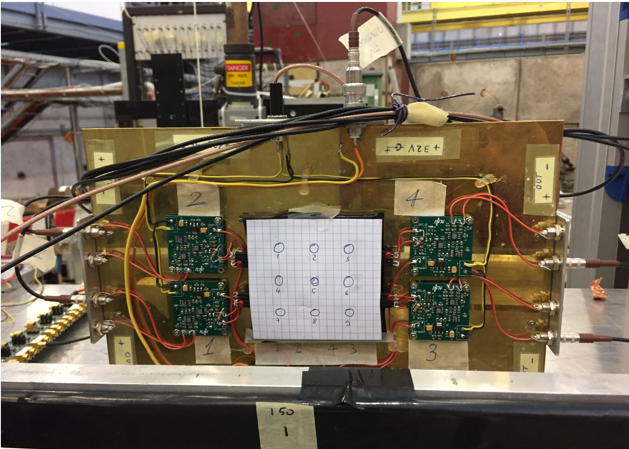
\includegraphics[width=0.45\columnwidth]{figs/DecaySpectrometer/tile_on_TB.png}
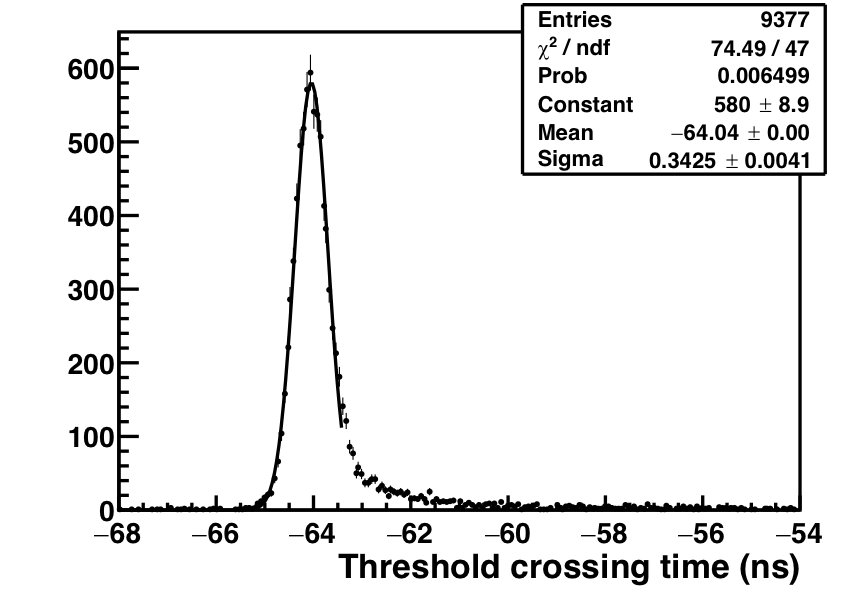
\includegraphics[width=0.45\columnwidth]{figs/DecaySpectrometer/time_reso.png}
\caption{Left: prototype of a tile for the muon system, tested at the T10 area, CERN-PS.
  Right: time resolution.}
\label{fig:tile}
\end{figure}
%
Scintillating tiles with direct SIPM readout is now the baseline solution for the SHiP Muon system.
The basic parameters of the system are summarized in Table~\ref{tab:muon_layout} assuming a preliminary tile dimension
of $10\times20\times1$ cm$^3$. The tiles geometry has been implemented in the SHiP Monte Carlo
at the digitization level, where the tiles are simulated side by side without dead spaces (see Figure~\ref{fig:muon_system}, right).
The choice of having the tiles at the digitization level and not hard-coded in the GEANT geometry
is driven by the request of having a geometry very flexible to be able to follow the upcoming test beam
results and the  evolution of the mechanical drawings of the system without rerun the (computationally heavy) GEANT simulation.
Given the excellent time resolution, the possibility of building the muon system with only three stations instead of four
is currently being considered and a final decision will be taken for the TDR.
% - table with main parameters:
\begin{table}[htbp]
\caption{Muon System layout as implemented in FairSHiP.}
\label{tab:muon_layout}
\vspace{.1cm}
\begin{center}
\begin{small}
\begin{tabular}{lr}
\hline
number of active stations  & 4 \\
active stations dimensions  & ($600 \times 1200 \times 1$) cm$^3$ \\
tile dimensions   & ($10 \times 20 \times 1$) cm$^3$ \\
number of tiles   &  3 600 $\times$ 4 = 14,400\\
weight of the scintillator & 11.52 t \\
FEE channels      &  14, 400 \\ \hline
number of passive iron filters   & 3 \\
filters dimensions  & $ (600 \times 1200 \times 60) $ cm$^3$ \\
iron weight   & $\sim$1000 t \\
\hline
\end{tabular}
\end{small}
\end{center}
\end{table}


\subsection{Detector performance}
\label{DSperformance}


%\begin{figure}[htb]
%\centering
%\includegraphics[width=0.9\linewidth]{figs/XXXXX.pdf}
%\caption{}
%\label{fig:XXXXX}
%\end{figure}